\documentclass[letter]{article}
\usepackage[margin=1in]{geometry}
%\documentclass[10pt]{article}
\usepackage[final]{graphicx}
\usepackage{color}
\usepackage{listings}
\usepackage{wrapfig}

%\usepackage[cm]{fullpage}
\usepackage{
amsfonts,amssymb,
amsmath,
url,graphics,subfig,
cite,
calc,
psfrag, bm,
amsthm, 
paralist}

%\renewcommand{\textwidth}{5.5in}

%---- Some math. macro
\newcommand\infsum[1][n]{\ensuremath{\sum_{#1=-\infty}^\infty}}

% Here's the definition of Sb, stolen from amstex
    \makeatletter
    \def\multilimits@{\bgroup
  \Let@
  \restore@math@cr
  \default@tag
 \baselineskip\fontdimen10 \scriptfont\tw@
 \advance\baselineskip\fontdimen12 \scriptfont\tw@
 \lineskip\thr@@\fontdimen8 \scriptfont\thr@@
 \lineskiplimit\lineskip
 \vbox\bgroup\ialign\bgroup\hfil$\m@th\scriptstyle{##}$\hfil\crcr}
    \def\Sb{_\multilimits@}
    \def\endSb{\crcr\egroup\egroup\egroup}
\makeatother

\newtheoremstyle{t}         %name
    {\baselineskip}{2\topsep}      %space above and below
    {\rm}                   %Body font
    {0pt}{\bfseries}  %Heading indent and font
    {~}                      %after heading
    { }                      %head after space
    {\thmname{#1}\thmnumber{#2}.}

%\theoremstyle{t}
%\newtheorem{q}{Q}
\parindent=0pt 

\newtheorem{Lemma}{Lemma}
\newtheorem{prop}{Proposition}
\newtheorem{Theorem}{Theorem}
\newtheorem{Corollary}{Corollary}
\newtheorem{Claim}{Claim}
\newtheorem{Fact}{Fact}
\newtheorem{Observation}{Observation}
\newtheorem{Assumption}{Assumption}


\theoremstyle{remark}
\newtheorem{Remark}{Remark}
\newtheorem{Example}{Example}


\begin{document}

\setcounter{page}{1}
\linespread{1.1}
\normalsize

\setlength{\parskip}{.2cm}

\begin{center} {\Large \textbf{
Opinion Dynamics with  reluctant agents} \vspace{.3cm} \\
{\normalsize ---~an ECS289F Project (Spring 2014)~---}} \vspace{.3cm}

{Hoi-To Wai, Christopher Patton}

\today

\end{center}
\vspace{0.1cm}


\begin{abstract}
The study of opinion dynamics attempts to model and predict the evolution of opinions in social networks. Pioneered by DeGroot and many others, previous works have studied scenarios where the opinion updates are non-linear, when the agents are heterogenous, etc. 
We propose a variation of the DeGroot model which attempts to capture \emph{reluctance} in agent behavior. Specifically, we study the affects of reluctant agents on opinion dynamics using mathematical analysis and numerical simulations. We show that the opinions of agents converge to a consensus asymptotically. However, it is observed that such consensus value will no longer be the original average opinion held by the agents in the network. Instead, the consensus value on average will be biased towards the initial opinion held by these reluctant agents. This suggests that the social network may fail to attain the `wisdom of the crowd'. 
Finally, we present several extensions to the described model. 
\end{abstract}


%-----------------------------------------------------------------------------
%\vspace{0.5cm}

\section{Introduction} \vspace{-.3cm}

Modelling the social network accurately is one of the major thrusts in the study of network science. A popular issue is to study the opinion evolution and how the social networks can lead to consensus (or to polarization) through local interactions among individuals. 

The study of opinion dynamics can be traced back to the 1970s, where DeGroot  first proposed a model to describe how consensus might be reached among a group of connected individuals \cite{Degroot_74}. In this model, every individual exchanges opinion with his/her neighbour and updates his/her opinion by computing the weighted average. The strength of the model lies on its simplicity and plausible description of the social network. 

Extensions to the DeGroot's model have been studied with the aim of strengthening the model by incorporating additional constraints. For example, \cite{Hegselmann02} studied opinion dynamics with bounded confidence such that the agents exchange opinions only with other agents that hold similar opinions, this model leads to a polarization in the final opinions held by the agents; \cite{Holley1975} studied the case when the opinions are discrete variables; \cite{Acemoglu2013,Yildiz2011} studied a special type of agents called the stubborn agents and \cite{Nedic2010} studied delayed consensus, etc.
In addition, the study of opinion dynamics is related to epidemic spread, the latter can be treated as a special case of discrete opinion dynamics. We also refer to \cite{Fagnani2014} for a recent tutorial-style overview on various opinion dynamics models and \cite{Das2014} for an experiment-based study. 

Besides the above extensions, the opinion dynamics model has inspired the creation of several decentralized algorithms in sensor networks. For example, algorithms that are inspired by the above opinion dynamics models have been successfully applied in various settings \cite{Dimakis2010}. 

However, most of the cited works above have ignored the fact that individuals may have different \emph{adaptation rates} of their neighbors' opinions. In light of this, we propose a novel kind of \emph{reluctant} agents. Here, instead of changing their opinion \emph{instantaneously}, the \emph{reluctant} agents slowly adapt to the `new' opinion at a certain rate.
In this regard, our work is closely related to the study of stubborn agents in \cite{Acemoglu2013}. Specifically, the \emph{reluctant} agent can be seen as a generalization of stubborn agents. 

Our project focuses on studying the behavior of these reluctant agents and their affects on social networks.
More precisely, we address the following issues: i) despite the departure from standard DeGroot's model, can consensus still be reached in the social network with the inclusion of reluctant agents? ii) if consensus can be reached, what will the consensus value be? iii) what is the effect if reluctant agents are placed strategically in the network?

The project report is organized as follows. Section~2 provides a mathematical description on the system model and introduces the novel reluctant agent model. Section~3 presents a convergence analysis on the opinion dynamics with reluctant agents. Section~4 validates the results in Section~3 using numerical simulations. 


\section{System model}
This section introduces the mathematical models used in opinion dynamics. We shall begin with the classical DeGroot model and then introduce the novel reluctant agent extension. 

Consider a social network modelled as an undirected graph $G = (V,E)$. There are $|V| = n$ agents and the edge set $E$ describes the relationships between the agents. 
We model the opinion held by each agent as a probability vector $\bm{w}_i \in \mathbb{R}^L$, i.e., it satisfies
\[
{\bf 1}^T \bm{w}_i = 1,~{\bm w}_i \succeq {\bf 0}.
\]
We consider a discrete time model. 
At time $t = 0$, each agent $i \in V$ holds an initial opinion ${\bm w}_i^{(0)} \in \mathbb{R}^L$. At time $t = k$ the opinion dynamics is described by:
\begin{equation}\label{eq:op}
\hat{\bm w}_i^{(k)} = \sum_{j \in \mathcal{N}_i} A_{ij}^{(k)} {\bm w}_j^{(k-1)},
\end{equation}
where $\hat{\bm w}_i^{(k)}$ is the weighted average opinion between the $i$th agent and its neighbor and $0 \leq A_{ij}^{(k)} \leq 1$ models the trust agent $i$ has on agent $j$ at time $k$. Importantly, we assume $\bm{A}^{(k)}$ is stochastic such that $\sum_{j=1}^{|V|} A_{ij}^{(k)} = 1$. Notice that the matrix ${\bm A}^{(k)}$ is time-variant and it is randomly generated at each $k$. 

In the DeGroot's model, the weighted average opinion is adopted \emph{immediately} by the agents:
\begin{equation} \label{eq:adapt_dg}
{\bm w}_i^{(k)} = \hat{\bm w}_i^{(k)}.
\end{equation}
We classify the agents following this rule \eqref{eq:adapt_dg} as \emph{normal} agents.

%It is known 
Observe that $\bm{A}$ is stochastic. Now, using Markov chain theories and under some other mild assumptions, it is not difficult to see that the dynamics \eqref{eq:op} converges such that
\[
{\bm w}_i^{(k)} = {\bm w}_j^{(k)},~\forall~i \neq j~{\rm as}~k \rightarrow \infty.
\]
Moreover, if $\bm{A}$ is also doubly stochastic such that $\sum_{i=1}^{|V|} A_{ij}^{(k)} = 1$, then the opinions converges to an average of the original one, i.e.,
\[
\lim_{k \rightarrow \infty} {\bm w}_i^{(k)}  = \frac{1}{n} \sum_{i \in V} {\bm w}_i^{(0)}.
\]
In fact, this is the situation that captures our attention as the opinions of the individuals will eventually converge to the \emph{`wisdom of the crowd'}. We believe that this is a desired situation in social networks, and in considering variations on this basic model, we assert this as our consensus goal.

A particular setup that gives a doubly stochastic matrix ${\bm A}$ is the so-called \emph{randomized gossip model} \cite{Boyd2006}. 
This model is designed to mimic the `gossiping' interaction between individuals. In particular, at each time, only two individuals talk to each other and the others are silent. 
Mathematically, the corresponding mixing matrix ${\bm A}^{(k)}$ is given as:
\[
{\bm A}^{(k)} = {\bf I} - \frac{1}{2} ({\bf e}_i + {\bf e}_j) ({\bf e}_i + {\bf e}_j)^T,
\]
where $(i,j) \in E$ is an edge of $E$ selected uniformly and independently at time $k$. 
%The model represents the scenario when agents communicate by `gossiping', i.e., at each time there can only be two agents exchanging idea with each other. 
It is obvious that ${\bm A}^{(k)}$ is doubly stochastic and such dynamics finds the `wisdom of the crowd'. 

%The vector $\hat{\bm w}_i^{(k)}$ is the opinion that agent $i$ is supposed to hold at time $k$. In DeGroot's model, the agents are updating instantly such that ${\bm w}_i^{(k)} = \hat{\bm w}_i^{(k)} $. In this case, it is known that ${\bm w}_i^{(k)}$ converges to the average of $\{{\bm w}_i^{(0)} \}$ asymptotically, i.e., achieving the `wisdom of the crowd',  under some mild assumptions. 
%For instance, the result can be easily obtained by exploiting the property that the sequence of random matrice $\{ {\bm A}^{(k)} \}$ is an independent process. 

In the above model, we observe that the opinions are updated \emph{instantly} when the individual interacts. In the socio-economical settings, some agents may be unwillingly to accept new ideas immediatedly. Instead, certain agents may be `reluctant' to adapt to its neighbor's idea. In the following sections, we discuss two types of agents that obey a different adaptation rule than \eqref{eq:adapt_dg}. 

\subsection{Stubborn agents} 
The stubborn agents model has been studied in \cite{Acemoglu2013}. Simply speaking, these are the agents who will \emph{never} update their opinion, i.e.,
\begin{equation} \label{eq:adapt_stubborn}
{\bm w}_i^{(k)} = {\bm w}_i^{(k-1)}.
\end{equation}
Such adaptation rule models the case when an individual is never going to change his/her opinion. We believe that this may be too extreme in a social network. This inspires us to propose the following reluctant agent model. 

\subsection{Reluctant agents}
We consider a new type of agent called the `reluctant' agent. In particular, these are the agents who do not update \emph{immediately}. We associate each reluctant agent with an adaptation rate of $\tau_i$. Then, ${\bm w}_i^{(k)}$ will be updated by:
\begin{equation} \label{eq:adapt}
{\bm w}_i^{(k)} = \frac{\min\{ c_i^{(k)}, \tau_i\} }{\tau_i} \hat{\bm w}_i^{(k - c_i^{(k)} + 1)} + \frac{\tau_i - \min\{ c_i^{(k)}, \tau_i\} }{\tau_i} {\bm w}_i^{(k-c_i^{(k)})},~i \in V_r,
\end{equation}
where $V_r \subseteq V$ is the set of reluctant agents, $c_i^{(k)}$ is a counter variable such that
\[
c_i^{(k)} = \begin{cases}
1 &,~{\rm if}~A_{ij}^{(k)} \neq 0,~\text{for some}~j \in V~\text{(agent $i$ talked at time $k$)}. \\
c_i^{(k-1)} + 1 &,~{\rm otherwise}
\end{cases}
\]
and $\tau_i \in \mathbb{Z}$ is the adaptation rate of $i$. From \eqref{eq:adapt}, it is important to clarify the mechanism that reluctant agent updates: i) the reluctant agent will slowly adapt to the new opinion in $\tau_i$ time steps; ii) if the agent is `interrupted' during the adaptation process, it will \emph{restart} the adaptation process based on ${\bm w}_i^{(k-1)}$. As an analagy, it is typical to take time to consider an idea in the context of your current opinion; when a new suggestion presents itself, one may set aside the previous one and focus on the new one. In a sense, our relcutant agent is greedy in his adaptation methodology.

We remark that the reluctant agent model offers a trade-off between normal and stubborn agents. Specifically, if $\tau_i = 1$, then agent $i$ is a normal agent; and if $\tau_i = \infty$, then agent $i$ is a stubborn agent. 

%We shall discuss the motivation and possible extensions/applications of the above model towards the end of this report.

%\subsection{Project goal and deliverables} 

%\subsection{Previous works and references} 
%Our work is based upon the pioneering paper by DeGroot \cite{Degroot_74} and a recent survey in \cite{Fagnani2014} (and the references therein). Furthermore, the reluctant agent model is inspired by \cite{Acemoglu2013}, which has studied the effect of \emph{stubborn} agents in a social network. For the simulation, we may also follow the reference \cite{Das2014} which has conducted experiments on opinion dynamics using real data. 
%
%While we are conducting the convergence analysis, we found that the references \cite{Nedic2010} have provided a nice framework for us to develop our theories. In particular \cite{Nedic2010} has considered and analyzed a delayed consensus model. In addition, the recent result from \cite{Touri2014} will also be applied in the analysis. 


%For the convergence analysis, 


\section{Convergence Analysis} 
In this section, we perform a convergence analysis for the proposed opinion dynamics model with reluctant agents. 
The main result is that we can establish that the opinions will  converge to a (biased) consensus almost surely. 
Furthermore, the converged opinion will be biased towards the initial opinions of the reluctant agent in expectation. 

We shall make the following assumption on the choice of mixing matrix ${\bm A}^{(k)}$:
\begin{Assumption}
Let $\mathcal{M}_k \subseteq E$ denote the subset of edges active at time $k$. Also, $\mathcal{M}_k \cup \mathcal{M}_{j}$ denotes the composite edge set such that if $(i,j) \in \mathcal{M}_k$ and $(j,k) \in \mathcal{M}_j$, then $(i,j),(j,k),(i,k) \in \mathcal{M}_k \cup \mathcal{M}_{j}$. The following events hold with probability one:
\begin{enumerate}
\item The composite graph $(V, \cup_{\ell = \ell'}^\infty \mathcal{M}_\ell)$ is fully connected for all $\ell' > 0$. 
\item For all $i,j \in V$, there exists a finite $L > 0$ such that $(i,j) \in \cup_{\ell = k}^{k+L-1} \mathcal{M}_\ell,~\forall~k.$
\end{enumerate}
\end{Assumption}
Roughly speaking, the above assumptions require ${\bm A}^{(k)}$ to be selected such that any two individuals in the network can (indirectly) exchange opinions infinitely often (as $k \rightarrow \infty$). 
As an example, we may consider the randomized gossip model on a graph such that there is a path between every pair of nodes. The mixing matrix ${\bm A}^{(k)}$ constructed  satisfies the above assumption.

%We propose to analyze our model under the framework of \cite{}. The latter reference has studied a delayed consensus model by considering an augmented system with a few extra nodes that models the delay in the system. The augmented system is delay-free and it can subsequently be analyzed. 
We shall now proceed with the convergence analysis. 
Our analysis is inspired by \cite{Nedic2010} and applies the result in \cite{Touri2014}. The main idea is to develop an equivalent model such that the modified opinion dynamics can be expressed as
\[
\tilde{\bm w}_i^{(k)} = \sum_{j=1}^{|V'|} \bar{A}_{ij}^{(k)} \tilde{\bm w}_j^{(k-1)}.
\]
We now consider a directed graph $G' = (V',E')$ where $V'$ contains all the nodes from $V$ together with $2|V_r|$ augmented nodes. 

For each $i \in V_r$, we define $2$ new nodes denoted by $\{ i', i'' \}$. Here, the $i'$th node stores the value of $\hat{\bm w}_i^{(k)}$ and the $i''$th node stores the value of old ${\bm w}_i^{(k)}$. The inter-connectivity of these nodes are best illustrated by the example in Fig.~\ref{fig:augment}. 

\begin{figure}[t]
\centerline{\resizebox{.5\textwidth}{!}{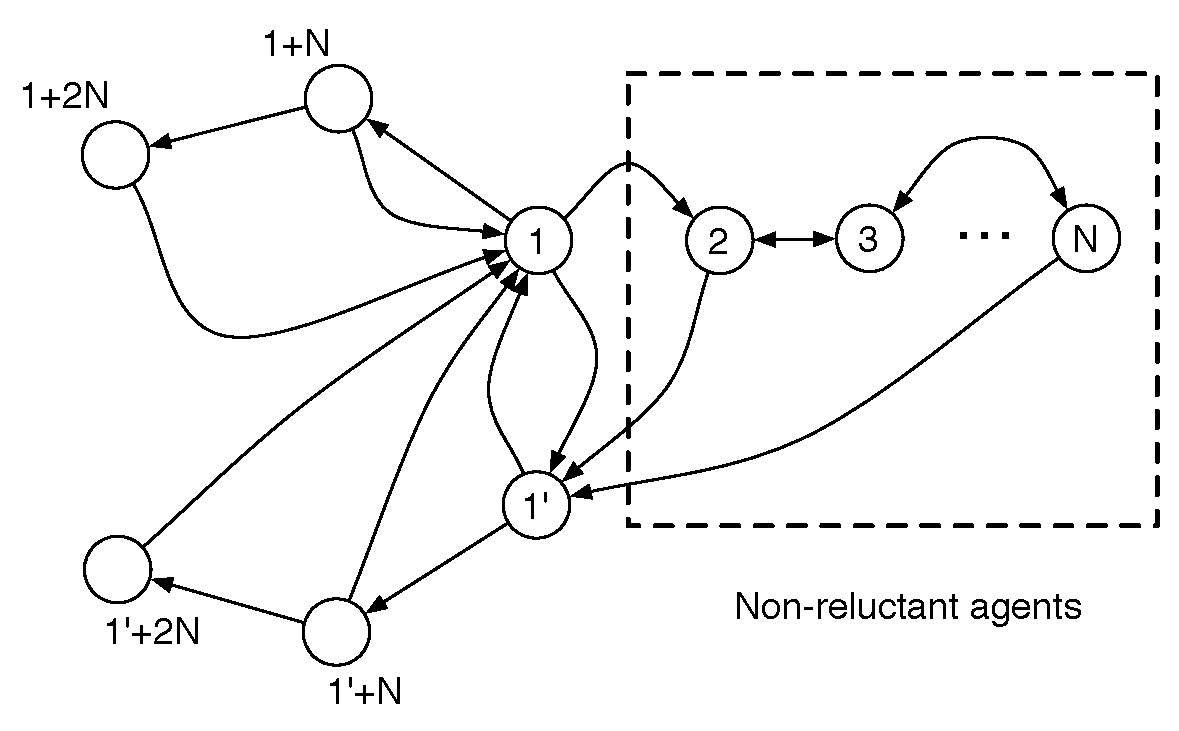
\includegraphics{./augmented_graph}}
}
\caption{Example of the augmented system for $V_r = \{1\}$. 
} \label{fig:augment}
\end{figure}

Using the augmented system $G'$, we can describe the equivalent opinion dynamics that executes on the graph. In particular, we split the update dynamics at time $k$ to two steps $k$ and $k'$. Step $k$ corresponds to the update stage \eqref{eq:op} and step $k'$ corresponds to the adaptation stage \eqref{eq:adapt}. 
Additionally, the counter variable $c_i^{(k)}$ is defined as before and they are updated before step $k$. 

Let $\tilde{ \bm w}_i$ be the opinion held by agent $i$ in the augmented system, the system is initialized as follows.
\[
c_i^{(0)} = M,~\forall~ i \in V'~{\rm and}~\tilde{ \bm w}_i^{(0)} = \begin{cases} { \bm w}_i^{(0)} &,~i \in V \\
 {\bf 0} &,~i \in V' \setminus V, \end{cases}
\]
where $M > \tau_i$ for all $i$ enforces a `reset' state for the adaptation process. 

\textbf{Updating stage}: At the \emph{updating} stage, we have that 
\[
\tilde{\bm w}_i^{(k)} = \sum_{j \in \mathcal{N}_i} A_{ij}^{(k)} \tilde{\bm w}_j^{(k-1)'},~i \in V \setminus V_r,
\]
i.e., the non-reluctant agents are updated immediately. 
As for node $i \in V_r$, we have $$\tilde{\bm w}_i^{(k)} = \tilde{\bm w}_i^{(k-1)'}$$ such that it is left intact. 
For node $i'$ where $i \in V_r$, we have:
\[
\tilde{\bm w}_{i'}^{(k)} = \begin{cases}
\displaystyle \sum_{j \in \mathcal{N}_i} A_{ij}^{(k)} \tilde{\bm w}_j^{(k-1)'}&,~{\rm if}~c_i^{(k)} = 1. \\
\tilde{\bm w}_{i'}^{(k-1)'}&,~{\rm otherwise},
\end{cases}
\]
and for node $i''$ where $i \in V_r$, 
\[
\tilde{\bm w}_{i''}^{(k)} = \begin{cases}
\tilde{\bm w}_{i}^{(k-1)'}&,~{\rm if}~c_i^{(k)} = 1. \\
\tilde{\bm w}_{i''}^{(k-1)'}&,~{\rm otherwise}.
\end{cases}
\]
The two equations above describes the opinion dynamics that when the counter variable $c_i^{(k)}$ is reset, then the stored variables will be updated. 

Let us define $\tilde{\bm A}^{(k)}$ as the overall updating matrix in this stage, i.e., we have:
\[
\tilde{\bm w}_i^{(k)} = \sum_{j=1}^{|V'|} \tilde{A}_{ij}^{(k)} \tilde{\bm w}_j^{(k-1)'}.
\]
It can be verified that $\tilde{\bm A}^{(k)}$ is stochastic. 

%Moreover, the updated opinion will be stored in the $i'$th node if $i$ is a reluctant agent:
%\[
%\tilde{\bm w}_{i'}^{(k)} = \sum_{j \in \mathcal{N}_i} A_{ij}^{(k)} \tilde{\bm w}_j^{(k-1)'},~i \in  V_r,
%\]
%The opinions at the other augmented nodes are updated as follows:
%\[
%\tilde{\bm w}_{i+j N}^{(k)} = \tilde{\bm w}_{i + (j-1)N}^{(k-1)'},~j=1,...,\tau_i - 1,~i \in V_r,
%\]
%\[
%\tilde{\bm w}_{i' +j N}^{(k)} = \tilde{\bm w}_{i' + (j-1)N}^{(k-1)'},~j=1,...,\tau_i - 1,~i \in V_r.
%\]
%To summarize, let us define $\tilde{\bm A}^{(k)}$ as the updating matrix in this stage, we have:
%\[
%\tilde{\bm w}_i^{(k)} = \sum_{j=1}^{|V'|} \tilde{A}_{ij}^{(k)} \tilde{\bm w}_j^{(k-1)'}
%\]
%where $\tilde{\bm A}^{(k)}$ is:
%\begin{equation} \label{eq:a_update}
%\tilde{A}_{ij}^{(k)} = \begin{cases}
%A_{ij}^{(k)} &,~i \in V \setminus V_r, \\
%A_{ij}^{(k)} &,~i = i', \\
%1 &,~i = j~{\rm and}~i \in V_r,\\
%1 &,~i = m + \ell N,~j=m + (\ell-1) N~{\rm for~some}~m \in V_r, \\
%1 &,~i = m' + \ell N,~j=m' + (\ell-1) N~{\rm for~some}~m \in V_r, \\
%0 &,~{\rm otherwise}.
%\end{cases}
%\end{equation}

\textbf{Adaptation stage}: At the \emph{adaptation} stage, the non-reluctant agents and the augmented nodes will remain unchanged, i.e.,
\[
\tilde{\bm w}_i^{(k')} = \tilde{\bm w}_i^{(k)},~i \in V' \setminus V_r.
\]
However, the opinion of the reluctant agent will be adapted using the stored information in node $i'$ and $i''$:
\[
\tilde{\bm w}_i^{(k')} = \begin{cases}
\displaystyle \frac{c_i^{(k)}}{\tau_i} \tilde{\bm w}_{i'}^{(k)} + \frac{\tau_i - c_i^{(k)}}{\tau_i} \tilde{\bm w}_{i''}^{(k)} &,~{\rm if}~c_i^{(k)} \leq \tau_i, \vspace{.2cm} \\
\tilde{\bm w}_i^{(k)} &,~{\rm otherwise}.
\end{cases}
\]
With some efforts, the dynamics described above can also be written using an update matrix $\tilde{\bm A}^{(k')}$. Such $\tilde{\bm A}^{(k')}$ is also found to be stochastic.

To summarize, we can now write the opinion dynamics as:
\[
\tilde{\bm w}_i^{(k')} = \sum_{j=1}^{|V'|} \tilde{A}_{ij}^{(k')} \sum_{\ell=1}^{|V'|} \tilde{A}_{j \ell}^{(k)} \tilde{\bm w}_{\ell}^{(k-1)'} =  \sum_{j=1}^{|V'|} \bar{A}_{ij}^{(k)} \tilde{\bm w}_{j}^{(k-1)'},
\]
where $\bar{\bm A}^{(k)} = \tilde{\bm A}^{(k')}  \tilde{\bm A}^{(k)}$ is a stochastic matrix. 

%We are interested in . 
%It turns out that the result is not trivial to obtain. 
We now analyze the convergence properties of the above model.
The main challenge is that the update matrix $\bar{\bm A}^{(k)}$ is correlated with its previous realizations, e.g., $\bar{\bm A}^{(k-1)}, ..., \bar{\bm A}^{(1)}$. 
However, using a recent result from \cite{Touri2014}, we are able to prove the following. 
%To prove the main result of the convergence analysis, we apply a recent result from \cite{}. 

Define 
\[
\bm{\Phi} (s+t,s) = \bar{\bm A}^{(s+t)}  \bar{\bm A}^{(s+t-1)} \ldots  \bar{\bm A}^{(s)}
\]
We have the following claim:
\begin{Claim}
${\bf \Phi} (k+t,k)$ is a stochastic matrix for all $k$. Moreover, there exists $\eta, t > 0$ such that:
\begin{equation} \label{eq:claim}
E \left( [{\bf \Phi} (k+t,k)]_{ij} | \mathcal{F}_{k} \right) \geq \eta E \left( [{\bf \Phi} (k+t,k)]_{ji} | \mathcal{F}_{k} \right),~\forall~i,j,k,
\end{equation}
where $ \mathcal{F}_{k}  = \{  \bar{\bm A}^{(k-1)},  \bar{\bm A}^{(k-2)}, ...,  \bar{\bm A}^{(1)} \}$ denotes the events that happened in the past (prior to the $k$th time step). 
\end{Claim}
%As coined in \cite{}, the opinion dynamics of our model is called a \emph{balanced} process
%The result can be applied as follows. 

%A rigorous proof for this claim is more technical and will not be pursued here. 
%To gain some insights, if we assume that the original graph $G$ is fully connected, then \eqref{eq:claim} can be satisfied for $t = 2$. The reason is that there is a non-zero probability for any two nodes  in the augmented system to communicate with each other in 2 hops. A   rigorous proof is provided as follows:

\textbf{Proof.} 
We claim that \eqref{eq:claim} can be achieved by setting $t = L$. 

This is based on a simple observation. When conditioned on ${\cal F}_k$ and under Assumption~1, there is a non-zero probability that any two nodes in the augmented system are connected in the resultant composite graph over an epoch of length $L$. As such, the expectation satisfies $$E( [{\bf \Phi} (k+t,k)]_{ij} | {\cal F}_k ) > 0,~\forall~i,j \in V'$$
for all $k$. 
%In particular, (conditioned on ${\cal F}_k$) we only need to verify that there exists a realization of ${\bf \Phi}$ that contains only non-zero entries; and this realization happens with non-zero probability. Such realization can be constructed under the assumptions. 

Now, let $\rho_{min} = \min_{i,j} E( [{\bf \Phi} (k+t,k)]_{ij} | {\cal F}_k ) > 0$ and we choose $\eta = \rho_{min}$. We observe that \eqref{eq:claim} can be satisfied as $0 < E( [{\bf \Phi} (k+t,k)]_{ij} | {\cal F}_k ) \leq 1$.~\hfill~{\bf Q.E.D.}

As a consequence of the above claim, the opinion dynamics with reluctant agents satisfies the so-called \emph{balancedness} property in \cite{Touri2014}. We have:
\begin{prop}
As the reluctant update model constitutes a balanced process, the opinions in reluctant updates model reach consensus almost surely, i.e., we have
% in the expectation as $k \rightarrow \infty$. We have
\begin{equation} \label{eq:propo}
\lim_{k \rightarrow \infty} P \left( \prod_{\ell=1}^{k} \bar{\bm A}^{(\ell)} = {\bf 1} ({\bm \pi}^\star)^T \right) = 1,
\end{equation}
for some ${\bm \pi}^\star \in \mathbb{R}^{|V'|}$ and ${\bf 1}^T {\bm \pi}^\star = 1$.
\end{prop}

The proof for Proposition~1 is skipped as it is a direct consequence of \cite{Touri2014}.
%{\color{red} I haven't looked into the proof of the theorem in \cite{} yet.} 
Proposition~1 implies that the dynamic model with the reluctant agents still reaches a consensus asymptotically. However, it is likely that the consensus reached will be biased, i.e., it differs from the true average. Notice that this happens when ${\bm \pi}^\star \neq {\bf 1} / |V'|$. In the subsequent analysis, we shall evaluate the magnitude of such bias empirically. 

%To obtain the desired result, we observe  that if ${\bm A}^{(k)}$ is stochastic, then $\tilde{\bm A}^{(k)}$ is also stochastic. To summarize, we have:
%\begin{prop}
%%Assuming that $\{ {\bm A}^{(k)} \}$ constitutes a sequence of opinion updates that lead to  consensus in the DeGroot's model as $k \rightarrow \infty$, then 
%The opinions in reluctant updates model reach consensus in the expectation as $k \rightarrow \infty$. We have
%\[
%\lim_{k \rightarrow \infty} E \left\{ \prod_{\ell=1}^{k} \tilde{\bm A}^{(\ell')} \tilde{\bm A}^{(\ell)} \right\} = {\bf 1} ({\bm \pi}^\star)^T,
%\]
%for some ${\bm \pi}^\star \in \mathbb{R}^{|V'|}$.
%\end{prop}

\subsection{Insights from the analysis using numerical simulations} \label{sec:bias}
We are interested in estimating the value of $E [ \bm{\pi}^\star ]$ in \eqref{eq:propo}. As mentioned before, evaluating the expected value analytically is non-trivial as the chain $\{ \bar{\bm A}^{(k)} \}$ is not independent. Here, in the interest of time, we only perform numerical simulations to estimate $E [ \bm{\pi}^\star ]$. As we shall see, this analysis shows that the system is biased towards the (initial) opinions of the reluctant agents. 

We consider a fully connected network with $N=10$ agents. There are $|V_r| = 2$ reluctant agents which are the first two agents in the system. Moreover, we have $\tau_1 = \tau_2 = 20$. 
We constructed the corresponding augmented graph and  evaluate the corresponding $E[\bm{\pi}^\star]$ (by averaging over 1000 Monte-Carlo trials). The results is as follows:
\[
E[\bm{\pi}^\star] = \left[  {\bf 0.2560~0.2521}~0.0616~ 0.0613~0.0607~0.0619~0.0610~ 0.0606~0.0626~0.0621~0~0~0~0 \right],
\]
where the last 4 entries corresponds to the augmented nodes. Moreover, if we consider the less reluctant agents, i.e., $\tau_1 = \tau_2 = 2$, we have:
\[
E[\bm{\pi}^\star] = \left[  {\bf 0.1095~0.1081}~0.0978~0.0975~0.0980~0.0980~0.0980~0.0978~0.0978~0.0976~0~0~0~0 \right].
\]

There are two observations we can draw from the above analysis. Firstly, instead of converging to an all-equal vector, $E[\bm{\pi}^\star]$ has  a heavier weight on the reluctant agents. This confirms that there is a bias associated with the network composed of reluctant agents. Secondly, the more \emph{reluctant} the agents are, the higher the bias. This is a reasonable result as the reluctant agents have higher chance to influence the others simply due to the fact that they are reluctant. 

The above observation also leads to a \emph{bias-equalization} approach that tries to cancel the bias induced by the reluctant agent. In particular, we may initialize ${\bm w}_i^{(0)}$ by:
\[
({\bm w}_i^{(0)})' = \frac{{\bm w}_i^{(0)}}{ (E[\bm{\pi}^\star])_i }
\]
However, such an approach may not work if we also look at the second order statistics of $\bm{\pi}^\star$. That is, we evaluate $\sigma_i = \sqrt{E[ (\pi_i - E[\pi_i])^2 ]}$. For $\tau_1 = \tau_2 = 20$, we have
\[
\bm{\sigma} = \left[  {\bf 0.0566~0.0535} ~0.0186~0.0167~0.0176~0.0184~0.0175~0.0163~0.0172~0.0181~0~0~0~0 \right],
\]
and for $\tau_1 = \tau_2 = 2$, we get
\[
\bm{\sigma} = \left[  {\bf 0.0137~0.0146} ~0.0075~0.0079~0.0078~0.0078~0.0074~0.0079~0.0078~0.0076~0~0~0~0 \right],
\]
In both cases, we observe that the standard deviation of $\bm{\pi}^\star$ is rather high. 

%To summarize, we believe that the results above are reasonable as the reluctant agents have higher chance to influence the others. One may 

\section{Simulation Studies}
This section describes a simulation study on the reluctant agent model. Our aim is to validate the analysis in the previous section and to inspire our future work.\footnote{The code is written in Python and uses the igraph library. It is avaialbe at \texttt{https://github.com/cjpatton/289f}.}
%In order to validate this analysis, and to inspire our further work, we wrote a program to simulate the reluctant agent model.
The goal of this work is to implement various asynchronous opinion dynamics models, including symmetric gossip, asymmetric gossip, and broadcast, as described in \cite{Fagnani2014}. We also hope to support easily customizable agent types. This gives us the flexibility to consider different applications. 

Intuitively, we expect node centrality to be the primary factor in the bias caused by a reluctant agent; our results confirm this. Our tests involve a set of standard agents with initial opinion 1 and a single reluctant agent ($\tau = 50$) with initial opinion 100. We generated a 100-node Erdos-Renyi random graph and a 100-node Barabasi-Albert random grpah. We ran the simulation 5,000 times, assigning the reluctant agent to a random, fixed node in the ER graph, and the most central node in the Barabasi-Albert graph. 

\subsection{Consensus score}
We ran our simulations within the symmetric gossip exchange model. It is shown in \cite{Fagnani2014} that, although asynchronous, this process is still stochastic. Therefore, we expect the "wisdom of the crowd" -- i.e. the true average, 1.99 in our case -- to be reached in simulations with standard agents. (Simulations validate this assumption.)

In the presence of relcutant agents, we observe a significant bias in the score distribution in both of these scenarios. (See Figure 2 for full illustrattions.) In the ER case, we see a Poisson-like distribution to the consensus scores with a mean relatively close to the true avearage. In the BA case, where a highly central node was designated reluctant, we see a major bias centered around an approximate mean of 8.9. We can say conclusively that centrality is a major factor in consensus.

\begin{figure}[h]
  \begin{tabular}{cc}
    Erods-Renyi & Barabasi-Albert \\ 
    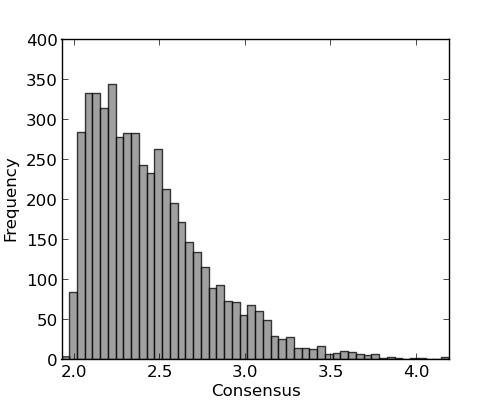
\includegraphics[scale=0.6]{figures/er_consensus.png} &
    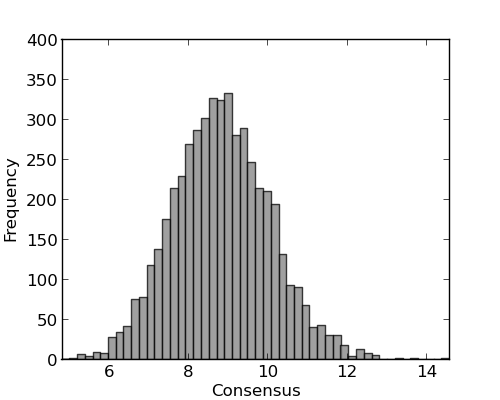
\includegraphics[scale=0.6]{figures/bar_consensus.png} \\
  \end{tabular}
  \caption{Distribution of consensus scores produced in the ER and BA random graphs (5,000 trials). The reluctant agent was chosen uniform randomly over the ER graph; in the BA network, the most central node was chosen. The true average is 1.99.}
\end{figure}

\pagebreak

%\begin{wrapfigure}{r}{0.5\textwidth}
\begin{figure}[h]
  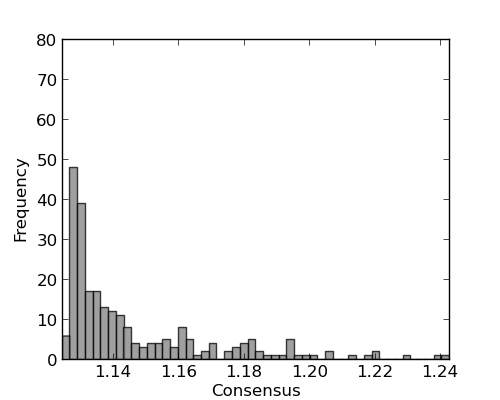
\includegraphics[scale=0.6]{figures/fb_consensus.png}
  \caption{Distribution of consensus scores for the social media data. Due to the high density of the graph, it was only computationally feasible to perform 250 trials. True average is 1.128.}
\end{figure}
%\end{wrapfigure}
In addition to these synthetic data, we retrieved some social network data\footnote{Available at \texttt{https://http://snap.stanford.edu/data/egonets-Facebook.html}.} obtained initially from Facebook. This test set consists of 768 nodes and 28,048 directed edges. The true consensus score in the standard model is 1.128. As before, we fixed one reluctant agent with initial opinion 100 and $\tau = 50$ to a node chosen uniform randmly; all others were standard agents with initial opinion 1. The distribution follows a similar pattern as the ER simulations. 

\subsection{Time to convergence}
We present the distribution of convergence times for our simulations. The time to convergence is defined as the number of rounds of symmetric goshe sip exchange until consensus was reached. Figure 5 in the appendix presents the results along with control experiments in which reluctant agents weren't used. Interestingly, the distributions didn't vary in a signficant way, except in the BA case when the most central node was chosen to be reluctant. (In this case the mean time to convergence differed by about 500 rounds.) The real world data contained an order of magnitude more edges than our synthecized data; thus, millions of exchanges were required before consensus could be reached. As a result, the adaption rate of $\tau = 50$ was completely swamped in our demonstrations. We cannot say conclusively whether the reluctant agent had an impact on time to convergence in this case, but we suspect that it may be analogous to the ER case. 


\subsection{\emph{Unbiased} reluctant agents}
When developing the simulation software for this project, we stumbled upon a variation of the reluctant agent model which, while impacting the time to convergence in the manner described above, had no biasing affect on the consensus score. The "wisdom of the crowd" was reached in all simulations. When a reluctant agent already adapting to a new opinion is engaged in a new exchange, it adapts to \emph{both} opinions simultaneously instead of dropping the old one. In the code, an exchange with a reluctant agent triggers an update in opinion on subsequent rounds equal to the average of the opinions divided by the adaption rate. In the standard reluctant agent model, a new trigger kills the previous one; in the variant on hand, all triggers are allowed to proceed simultaneously.\footnote{See classes \textit{ReluctantAgent} and \textit{UnbiasedReluctantAgent} in the code to see this distinction in practice.} 

We claim that the process remains doubly stochastic, and the true average is reached as a result. This could easily be proven following principles outlined in section 3 of this report. This observation is interesting to us, as it allows us to understand precisely where the bias in the reluctant agent model comes from, albeit from an an algorithmic point of view.


\section{Conclusion}
We may conclude from our preliminary simulation results that the bias in consensus is expected to be small when a node is reluctant with uniform probability. However, nodes with high centrality can have a major biasing affect, as demonstrated dramatically in the BA model. An interesting follow up to this project would be a formal treatment of the consensus bias with respect to the centrality of targeted nodes in the network. More validation would follow from identifying a highly central node in our social media data and run the simulation with it being the reluctant agent. 
We also expect to complete the analysis in Section~\ref{sec:bias} to evaluate the (mean) bias value towards the reluctant agent. 

Finally, we would like to extend the idea of reluctant agent beyond the \emph{continuous} opinion dynamics model that we have studied here. For instance, we may consider \emph{discrete} opinion dynamics when the opinions are modelled as binary variables. 


\pagebreak
\section{Appendices}

A few materials related to our simulations. 
\begin{figure}[h]
  \begin{tabular}{c c}
    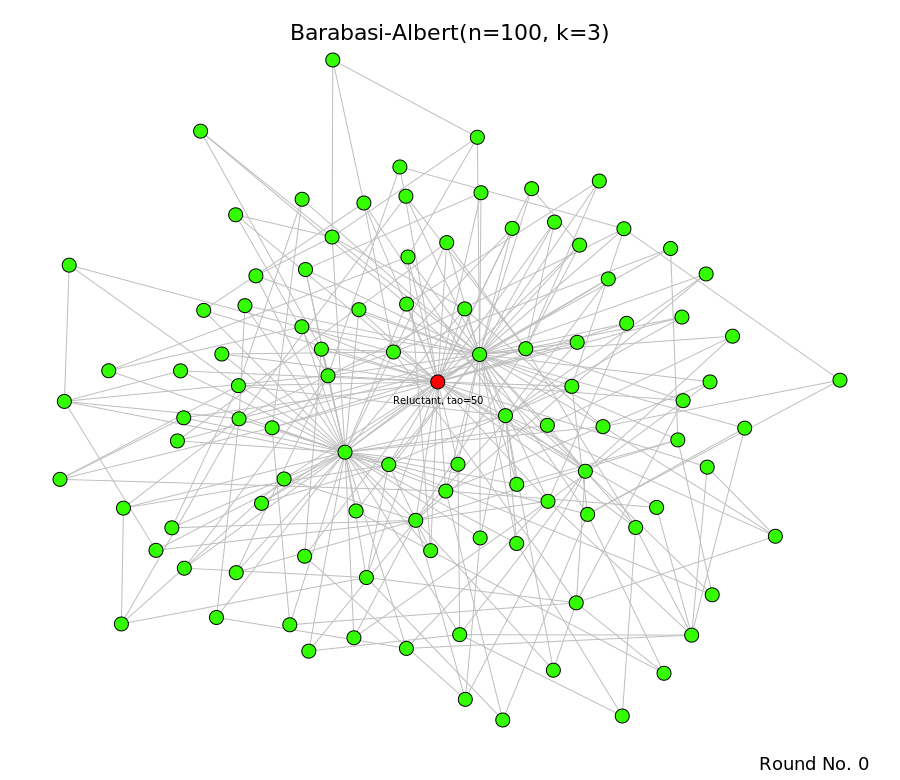
\includegraphics[scale=0.25]{figures/graph000000.png} &
    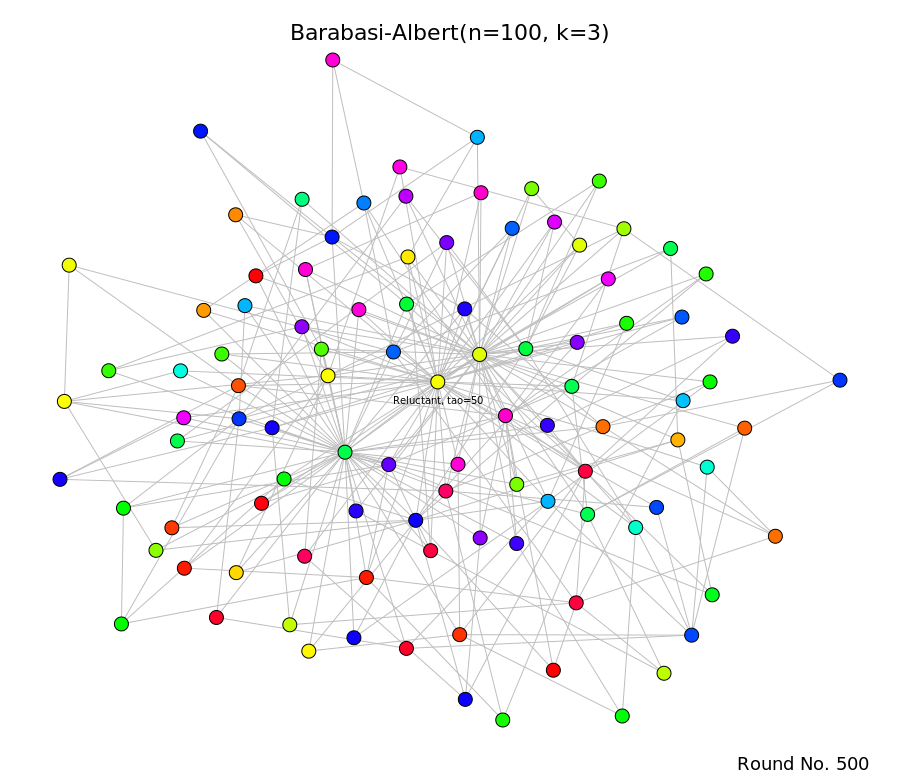
\includegraphics[scale=0.25]{figures/graph000500.png} \\ 
    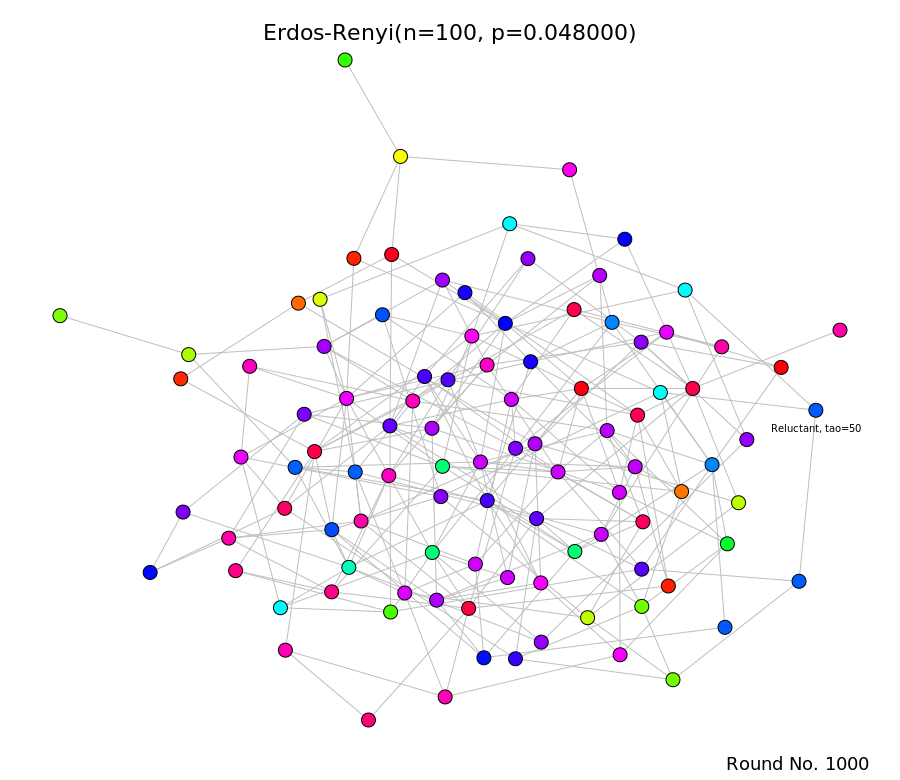
\includegraphics[scale=0.25]{figures/graph001000.png} &
    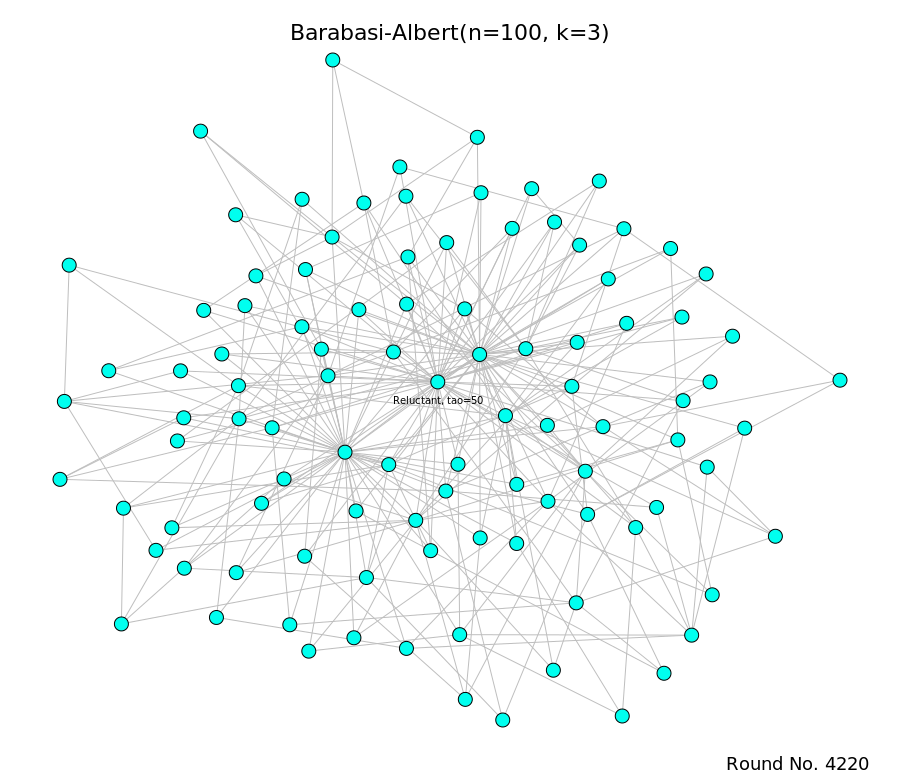
\includegraphics[scale=0.25]{figures/graph004220.png} 
  \end{tabular}
  \caption{An illustration of our simulation software in action. This is the Barabasi-Albert model described above, reaching consensus after 4,420 rounds. }
\end{figure}


\begin{figure}[]
  \begin{tabular}{c c}
    Reluctant agent & Control \\ 
    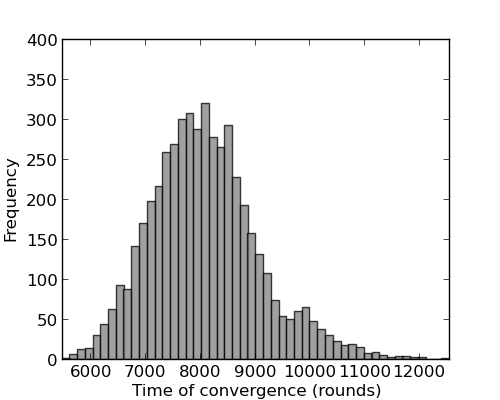
\includegraphics[scale=0.6]{figures/er_rounds.png} &
    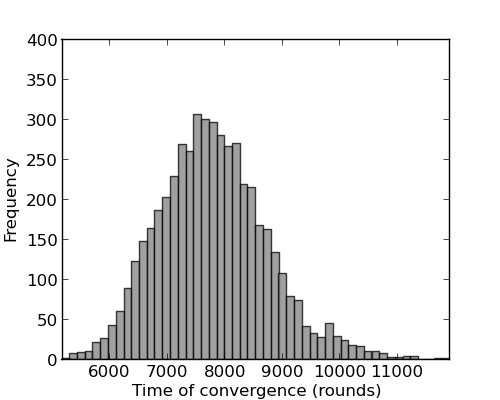
\includegraphics[scale=0.6]{figures/er_rounds_control.png} \\
    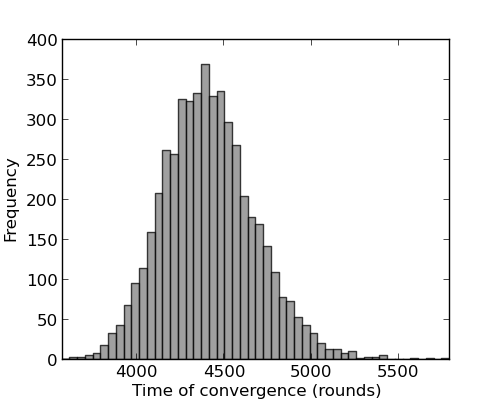
\includegraphics[scale=0.6]{figures/bar_rounds.png} &
    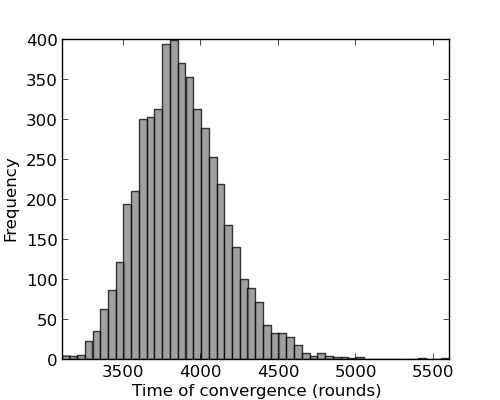
\includegraphics[scale=0.6]{figures/bar_rounds_control.png} \\
    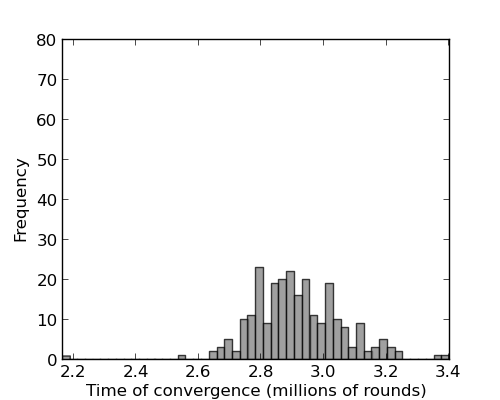
\includegraphics[scale=0.6]{figures/fb_rounds.png} &
    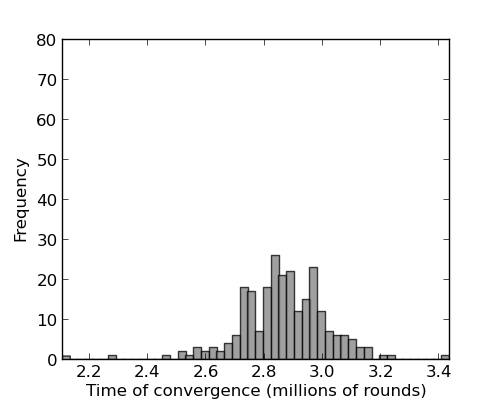
\includegraphics[scale=0.6]{figures/fb_rounds_control.png} \\
  \end{tabular}
  \caption{Consensus time distribution for all data sets. The top row correponds to ER, the middle to BA, and the bottom to the Facebook data. Those on the left contained a reluctant agent with initial opinion of 100; those on the right contained a normal agent instead, but still with initial opinion 100. While the consensus score was clearly biased in all scenarios, the time to convergence only shows significant bias when a highly central node is reluctant. } 
\end{figure}



%\lstset{
%  basicstyle=\small,
%  stringstyle=\ttfamily,
%  numbers=left,
%  numberstyle=\tiny,
%  stepnumber=1, 
%  numbersep=5pt,
%  language=Python }
%\lstinputlisting{figures/consensus.py}


\pagebreak
%\renewcommand{\refname}{\vspace{-1.5cm}}
%\small
\bibliographystyle{IEEEtran}
\bibliography{paper}


\end{document}
